% !TeX spellcheck = en_GB
\documentclass[10pt,letterpaper,oneside]{article}
\usepackage{fontspec}
\usepackage{arev}
\usepackage[utf8]{inputenc}
\usepackage[T1]{fontenc}
\usepackage{amsmath}
\usepackage{amsfonts}
\usepackage{amssymb}
\usepackage{graphicx}
\usepackage{csquotes}
\usepackage{booktabs}
\usepackage{multicol}
\usepackage{enumerate}
\usepackage{microtype}
\usepackage[labelfont=bf,font={small}]{caption}
\usepackage{hyperref}
\usepackage{booktabs}
\usepackage{subcaption}
\usepackage{fancyhdr}
\usepackage[svgnames]{xcolor}
\usepackage{mdframed}
\usepackage{multicol}
\usepackage[para]{footmisc}
\usepackage{siunitx}
\usepackage{cleveref}
\usepackage{listings}
\usepackage{cprotect}


\lstset{ % General setup for the package
	language=Python,
	basicstyle=\small\ttfamily,
	tabsize=4,
	columns=fixed,
	showstringspaces=false,
	showtabs=false,
	keepspaces,
	commentstyle=\color{SeaGreen},
	keywordstyle=\bf\ttfamily\color{DarkBlue},
	stringstyle=\ttfamily\color{Crimson}
}

\newfontfamily\symbolfont{Symbola}
\usepackage[left=1in,right=1in,top=1in,bottom=1in,marginparwidth=0.3in]{geometry}

\usepackage[sorting=none]{biblatex}
\addbibresource{../bibliography.bib}

\author{Andreas Stöckel\\[0.5cm]Based on lecture notes by\\Chris Eliasmith and Terrence~C.~Stewart}
\newcommand{\baseCodeURL}{https://github.com/celiasmith/syde556-w22/blob/master/lectures}

\fancyhf{}
\fancyhead[L]{SYDE 556/750 Lecture Notes}
\fancyhead[R]{Andreas Stöckel}
\fancyfoot[C]{\thepage}
\pagestyle{fancy}

\setlength{\parindent}{0em}
\setlength{\parskip}{0.5em}
\renewcommand{\baselinestretch}{1.25}

\renewcommand{\vec}[1]{{\mathbf{#1}}}
\newcommand{\mat}[1]{{\mathbf{#1}}}
\newcommand{\T}{\ensuremath{\mathrm{T}}}
\renewcommand{\epsilon}{\varepsilon}
\renewcommand{\phi}{\varphi}

\makeatletter
\newcommand{\superimpose}[2]{%
	{\ooalign{{#1}\hidewidth\cr{#2}\hidewidth\cr}}}
\makeatother
\newcommand{\SolidCircle}[2]{\superimpose{\color{#1}\symbolfont ⬤}{\textbf{\color{white}#2}}\hspace{1em}}
\newcommand{\OPlus}{\SolidCircle{DarkGreen}{\kern0.75pt+}}
\newcommand{\OMeh}{\SolidCircle{DarkOrange}{~}}
\newcommand{\OMinus}{\SolidCircle{DarkRed}{\kern2.25pt--}}

\newcommand{\YouTube}[2][Video]{\href{https://youtu.be/#2}{{\symbolfont 📺}~{#1}}%
%\footnote{\url{https://youtu.be/#2}}%
}

\newcommand{\CodeLink}[2][Code]{\href{\baseCodeURL/#2}{{\symbolfont ⌨}~\emph{#1}}}

\newcommand{\MakeTitle}[1]{
\maketitle
\begin{center}
	\includegraphics[width=0.5\textwidth]{../assets/uwlogo.pdf}\\[1cm]
	{#1}\
\end{center}

\vfill

\thispagestyle{empty}
\setcounter{page}{0}
\newpage

\pagenumbering{roman}
\setcounter{tocdepth}{2}
\tableofcontents
\newpage

\setcounter{page}{0}
\pagenumbering{arabic}}

\reversemarginpar


\newcommand{\ColorBox}[3]{%
	\marginpar{%
		\huge\raisebox{-3ex}{\symbolfont{#1}}%
	}%
	\begin{mdframed}[hidealllines=true,backgroundcolor=#2,innertopmargin=0.25cm,innerbottommargin=0.25cm]%
		{#3}
	\end{mdframed}}

\newcommand{\Note}[1]{\ColorBox{📌}{WhiteSmoke}{\textbf{Note:} #1}}
\newcommand{\Example}[1]{\ColorBox{💡}{WhiteSmoke}{\textbf{Example:} #1}}
\newcommand{\Aside}[1]{\ColorBox{🌟}{WhiteSmoke}{\emph{Aside:} #1}}
\newcommand{\Python}[1]{\ColorBox{🐍}{WhiteSmoke}{#1}}
\newcommand{\Notation}[1]{\ColorBox{\huge$\Sigma$}{WhiteSmoke}{\textbf{Notaton:} #1}}

\newcommand{\ConstructionSite}{\hrulefill {\symbolfont 🚧} UNDER CONSTRUCTION {\symbolfont 🚧} \hrulefill}

\newenvironment{ImportantEqn}[1]{\mdframed\raggedleft\emph{({#1})}\align}{\endalign\endmdframed}

\date{Fall 2022}
\title{SYDE 556/750 \\ Simulating Neurobiological Systems \\ Lecture 8: Learning}


\begin{document}

\MakeTitle{\textbf{Accompanying Readings: Chapter 9 of Neural Engineering}}

\section{Introduction}

\Note{As mentioned several times in previous lectures, we so far assumed that the connection weights between individual neuron populations are constant. This is of course not the case in biology, where animals change their behaviour in response to experiences sometimes years in the past.}

When talking about \emph{learning}, we should first define this term a little more rigorously. A very broad definition of learning from a neuroscientist's perspective (psychologists will have different definitions) could be \enquote{any process within a neural system that allows past stimuli to influence future behaviours}. Perhaps confusingly, this definition would also include dynamical systems that we have already talked about, such as integrators or the Delay Network.

In this course we will stick to a much more simple definition of learning:
\begin{mdframed}
	\hfill\emph{(Learning)}\\
	\emph{Learning} is a directed change in synaptic weights $\mat W$ while the network is active.
\end{mdframed}
Conversely, we refer to anything that fits into the category of \enquote{past-affecting-the-future} phenomena as \emph{adaptation}. Adaptation thus encompasses learning according to our definition, as well as dynamical systems, and short-term neural firing-rate adaptation.

Of course, now that we have defined what \enquote{learning} is, we should briefly discuss why this is a useful concept to talk about, especially within the Neural Engineering Framework. After all, we can already compute the \enquote{optimal} decoders, so why would we want to change those after the fact by changing the synaptic weights?

\begin{enumerate}[1.]
	\item \textbf{We might not know the function we want to compute at the beginning of a task.}\\
	Consider a simulated critter that explores its environment in search for food. Some food (the \enquote{green food}) is nutritious and should be eaten, whereas other food (the \enquote{red food}) is slightly poisonous and should be avoided.
	
	A priori, as modellers of this system, we might not know what awaits our critter in its environment. Hence, we have no chance to pre-compute the \enquote{correct} transformation that maps colour onto \enquote{edibility} of the foot. In fact, we might not even know which sensory modalities are important for this kind of decision (smell, colour, shape, taste, \textellipsis).

	If instead we were able to build a system that was able to \emph{learn} a mapping from sensory stimuli onto \enquote{edibility}, that might make our lives as modellers much easier.

	\item \textbf{The desired function might change over time.}\\
	Consider a dynamical system that controls joint muscle tensions for a given target position. While we may be able to build a system that performs this control efficiently when the system is first deployed, there may be several factors that change the required controller over time.

	For example, injury and ageing might cause wear in joints, growth (in a biological system) will change the lengths of the limbs, or the system may be required to handle loads that are much lighter or heavier than what was originally considered when designing the controller.

	\item \textbf{The \enquote{optimal weights} we are solving for are not optimal.}\\
	Remember that the synaptic weights $\mat W$ are defined as $\mat W = \mat E \mat D$ in a Neural Engineering Framework network. While the decoders $\mat D$ we are computing are optimal, this does not mean that the entire weight matrix $\mat W = \mat E \mat D$ is optimal! If we optimize the full weight matrix directly, this allows us to fit individual functions in a better way.
	
	Furthermore, at least when computing $\mat D$ using the rate-approximation $G[J]$, we are not taking the dynamics of the neurons into account. Remember that we derived $G[J]$ under the assumption of a constant, or static, input current $J$. Hence, the decoders $\mat D$ that are optimal in the \enquote{static} case are not necessarily optimal for the dynamics encountered in the neural network.

	\item \textbf{Answering scientific questions about learning in nervous systems.}\\
	As discussed in the lecture about transformations, our goal so far has been to build models of \enquote{expert systems}. We are trying to answer the question whether a system that has already learned to accomplish a certain task can be modelled by implementing certain mathematical transformations under optimal circumstances.

	Incorporating learning into our models allows us to answer a slightly different question, namely whether nervous systems with a certain overall connectivity can learn transformations from the stimuli that are available to it during its lifetime or growth (ontogenesis).
\end{enumerate}

These points should make it clear that incorporating learning into NEF networks is desirable. However, in order to do so, we will first take a short excursion to the field of Machine Learning, and have a glance at the types of \enquote{learning} usually employed by computer scientists (who, unfortunately, chose to not follow the definition of \enquote{learning} we made up above). We then apply some of these concepts, including supervised and unsupervised learning to biologically plausible neural networks.

\section{An Excursion to Machine Learning}

\begin{figure}
	\centering
	\includegraphics{media/learning_example_supervised.pdf}
	\caption{A supervised learning task. Given a set of $N$ examples mapping an image $\vec x_k$ onto a one-hot encoded category vector $\vec t_k$, we would like the computer to learn a mapping from unseen images $\vec x$ onto categories $\vec t$.}
	\label{fig:learning_example_supervised}
\end{figure}


Inspired by the learning abilities of biological systems, computer scientists and engineers have been working on \enquote{learning machines} since the early 1960s, giving rise to the uncreatively named field of machine learning. The main goal of this field is to apply computers to problems that have a less well-defined relationship between input and output.

\Example{Consider the following \enquote{image recognition} problem. A system receives an image encoded as a high-dimensional vector $\vec x$ (where each vector component corresponds to the intensity of one colour channel of a pixel in the image), and has to decide whether the image shows a dog, a cat, or a parrot (cf.~\cref{fig:learning_example_supervised}). It would be quite hard to write such a program \enquote{by hand}. After all, what are the rules by which we would categorize a mere bunch of pixels into these categories? The goal of machine learning is to be able to \enquote{program by example}. Instead of specifying an algorithm, we just specify examples, and the computer \enquote{figures out} (learns) on its own how to solve the problem in general.}

\newpage

Within this field, computer scientists typically distinguish between three types of learning:
\begin{itemize}
	\item \textbf{Supervised Learning}\\
	Given $N$ training samples $(\vec x_k, \vec t_k)$, and a model function $f(\vec x; \vec w)$, find weights/parameters $\vec w$ such that $f(\vec x_k) \approx \vec t_k$. We hope that after training, $f(\vec x; \vec w)$ will also work for unseen~$\vec x$. In other words, we assume that there is an unknown ground truth function $f_\mathrm{GT}(\vec x) = \vec t$ that we would like to approximate by tuning the parameters of our model function $f(\vec x; \vec w)$.\\
	\emph{Examples:} Polynomial fitting, Perceptrons, generalised linear models (GLMs), Support Vector Machines (SVMs), Gaussian Processes, Multi-Layer Perceptrons (MLPs).
	\item \textbf{Unsupervised (or Self-supervised) Learning}\\
	We are just given a set of $N$ samples $\vec x_k$ and would like to discover some inherent order within this dataset. Often, we would like to map each $\vec x_k$ onto a lower-dimensional \enquote{latent} space $\vec \lambda$, where conceptually similar $\vec x$ are being assigned to similar $\vec \lambda$. Self-supervised is often used to pick out examples where an error signal is internally generated. For example, large language models learn based on predicting masked words available in the training text.\\
	\emph{Examples:} Clustering, autoencoders, dimensionality-reduction methods (PCA, tSNE, \textellipsis).
	\item \textbf{Semi-supervised (or Reinforcement) Learning}\\
	A system receives state information $\vec x(t)$ and a low-dimensional reward signal $r(t)$. The goal is to learn a policy $\pi(\vec x)$ that produces actions $\vec t(t)$ maximizing the time-cumulative reward.
\end{itemize}

Furthermore, there are additional constraints on the learning process that are orthogonal to these concepts, such as \enquote{offline} (training happens while the system is not being used), \enquote{online} (the system learns on a stream of data), or \enquote{life-long} (the system is constantly learning whenever it is active, which is the type of learning we defined above) learning.

In the following sections, we have a closer look at these concepts. Maybe we can borrow some insights from Machine Learning and apply them to our spiking neural network models!

\section{Supervised Learning}

As summarized above, the goal of supervised learning is to find parameters $\vec w$ for a model function $f(\vec x; \vec w)$, such that the function closely maps a set of $N$ training data points~$\vec x_k$ onto a set of desired target points~$\vec t_k$. The quality of the match is defined according to some loss function $E(\vec w)$. For example, if we assume a quadratic loss function, a supervised machine learning problem could be phrased as
\begin{align}
	\vec w &= \arg \min_{\vec w} E(\vec w) = \arg \min_{\vec w} \frac{1}{N} \sum_{k = 1}^N \big\| f(\vec x_k ; \vec w) - \vec t_k \big\|^2 \,.
	\label{eqn:supervised_learning}
\end{align}
While equation \cref{eqn:supervised_learning} looks quite innocuous, this problem is generally difficult because of the function~$f$. There is no constraint whatsoever on what $f$ should look like, except for the very general notion of $f$ being a function mapping from a $d$-dimensional input space $\mathbb{X} \subseteq \mathbb{R}^d$ onto some $d'$-dimensional target space $\mathbb{R}^{d'}$. Commonly used examples of model functions $f$ include
\begin{itemize}
	\item Polynomial of degree $n$: $f(\vec x; \vec w) = \sum_{i = 0}^n w_i x^i$.
	\item Linear models: $f(\vec x; \vec w) = \sum_{i = 0}^n w_i \phi_i(x)$.
	\item Perceptron: $f(\vec x; \mat w) = \phi\big(\langle \vec w, \vec x \rangle \big)$.
	\item Multi-layer perceptrons/\enquote{deep} neural networks.
\end{itemize}

The overall goal of this endeavour is \emph{generalisation}. While our training tuples $(\vec x_k, \vec t_k)$ may only cover a small portion of the space $\mathbb{X}$ we are interested in, the general hope is that once we find the right parameters $\vec w$, our function $f(\vec x; \vec w)$ will also work for tuples $(\vec x_k, \vec t_k)$ we have not seen before. Underpinning this hope is the assumption that there exists a systematic mapping between $f_{\mathrm{GT}}(\vec x; \vec w)$ that is unknown to the engineer building the system, and that $f$ will approximate this $f_{\mathrm{GT}}$ after training.

Unfortunately, in general, there are not guarantees that this will actually work. To the contrary, we can guarantee that an algorithm solving for $\vec w$ that generalises well within one particular application domain will not be able to generalise in another application domain. This is known as the so-called \enquote{No Free Lunch Theorem}.

\Note{\emph{Solving for decoders is a supervised learning problem.}
The problem we solve when computing identity or function decoders fits exactly into this framework. In this case, our function $f(\vec x; \vec w)$ is just a linear model given as
\begin{align*}
	f(\vec x; \vec w) &= \langle \vec w, \vec a(\vec x) \rangle \,,
\end{align*}
where $\vec w$ are our decoders, and $\vec a(\vec x)$ is the function mapping from an input $\vec x$ onto the neural activities. As we saw, we can just solve for the optimal $\vec w$ using the $L_2$-regularised Moore-Penrose pseudo inverse.}

\subsection{Using Gradient Descent to Solve for $\vec w$}

\begin{figure}
	\centering
	\includegraphics{media/gradient_descent_poly_example_10.pdf}
	\caption{Gradient descent in action. We are trying to find parameters for the polynomial model function $f(x; \vec w) = w_0 x^2 + w_1 x$ given a set of samples $(x_k, t_k)$. \emph{Left:} Loss function over the parameters $\vec w$, as well as the trajectory of the paramters $\vec w$ as part of the gradient descent algorithm. Arrows indicate the gradient $\Delta \vec w$. Brighter colours correspond to larger errors. \emph{Right:} Training samples $(x_k, t_k)$, as well as the parametrised model functions corresponding to the parameters highlighted in the left picture. \CodeLink{lecture_08/media/code/gradient_descent_example.ipynb}}
	\label{fig:gradient_descent_poly_example_10}
\end{figure}

In general, it is impossible to solve for $\vec w$ in closed form. Instead, computer scientists often fall back onto a heuristic known as \enquote{gradient descent}.

In a nutshell, we analyse how infinitesimally small changes to one of the weights $w_i$ would affect our loss function $E(\vec w)$. We use this information in order to apply a small change $- \eta \Delta \vec w$ to our weights, such that the error is being reduced. In particular, this change is given as
\begin{align*}
	\Delta w_i &= \big( \nabla E(\vec w) \big)_i =  \frac{\partial E(\vec w)}{\partial w_i} = \frac{\partial}{\partial w_i} \frac{1}{N} \sum_{k = 1}^N \big\| f(\vec x_k ; \vec w) - \vec t_k \big\|^2 \,, & \text{weight update step } \vec w &\gets \vec w - \eta \Delta \vec w \,,
\end{align*}
where $\eta$ is the so called \emph{learning rate}. The weight update steps are then repeated until $\vec w$ converges (i.e.,~does not change considerably). See \cref{fig:gradient_descent_poly_example_10} for a simple example. Keep in mind that depending on $f(\vec x; \vec w)$, the loss function will not have a clear global minimum and the number of parameters can go into the billions (and not just two as in the example).

We can sometimes compute the partial differential $\frac{\partial}{\partial w_i}$ numerically (i.e., by evaluating $E$ for slightly different $\vec w$ and computing the difference quotient). For some $f$, the gradient $\nabla E$ can be evaluated efficiently using the chain-rule, leading to an algorithm called \emph{error back-propagation}. There are libraries such as Autograd or Tensorflow that conveniently compute these gradients.

In practice, the loss function $E$ is often not evaluated for all $N$ training samples at once, but for a random subset of $N' \ll N$ samples, where $N'$ is the so called \enquote{batch size}. Not only does this increase the efficiency of the gradient descent algorithm, it also prevents the algorithm from \enquote{getting stuck} in local minima. This variant of gradient descent is called \enquote{stochastic gradient descent} (stochastic because of the random selection of samples).

\subsection{The Delta Learning Rule}

As noted above, we are solving a supervised \enquote{learning} problem (in the machine learning sense) when computing decoders $\mat D$. However, so far we have been using what is known as an \emph{offline} method -- we compute $\mat D$ in one step for all $N$ using the $L_2$-regularised Moore-Penrose pseudo inverse. That is, we have a training phase during which we compute $\mat D$, followed by the \enquote{inference} phase during which we use $\mat D$ within our neural network.

In order to \emph{learn} synaptic weights $\mat W$ in the sense defined in the introduction, we need a so-called \emph{online} learning rule. That is, we would like to find a learning rule that allows us to update the weights for a stream of input data while the network is active.

Luckily, we can easily derive such an algorithm in two stages. First, we will implement a decoder learning rule by performing gradient descent for an input-target pair $(\vec x(t), \vec y^\mathrm{d}(t))$. This is somewhat comparable to stochastic gradient descent with a batch size of $N' = 1$, although we do not randomly sample from a pool of $N$ available samples, but always use the information that is currently (i.e., at time $t$) available in our network.

Second, we will extend this \emph{decoder} learning rule to a biologically plausible \emph{synaptic weight} learning rule that updates individual entries of the weight matrix $w_{ij}$.

For simplicity, let's assume that $d = 1$, i.e., we are representing a scalar value. Now, our setup is as follows. We have a neuron population representing the input value $x$ and would like to decode an unknown function $f(x)$. In other words, we would like to continuously update our decoders $\vec d$, such that $f(x(t)) \approx y^\mathrm{d}(t)$. This means that we have the following loss function
\begin{align*}
	E(\vec d) &= \frac{1}2 \left(\left(\sum_{i = 1}^n d_i a_i\big(x(t)\big) \right) - y^\mathrm{d}(t) \right)^2 \\
	\Rightarrow \Delta d_i = \frac{\partial E(\vec d)}{\partial d_i} &= \underbrace{\left(\left(\sum_{i = 1}^n d_i a_i\big(x(t)\big) \right) - y^\mathrm{d}(t)\right)}_{\epsilon(t)} a_i\big(x(t)\big) \\
		&= \epsilon(t) a_i\big(x(t)\big) \,,
\end{align*}
where $\epsilon(t)$ is the error we are making at the current point in time. This is a version of the so-called \enquote{Delta Learning Rule} for a linear model. In the next subsection we will extend this rule to individual synaptic weights $w_{ij}$.

\Note{Since we are not stochastically sampling from a large pool of $N$ samples, this method has a problem often referred to a \emph{catastrophic forgetting}. By not looking at older samples, we are temporarily over-fitting our system to the current region of the input-target space.}

\Aside{Stochastically sampling $(\vec x(t'), \vec y^\mathrm{d}(t'))$ pairs over a longer history $t' \in [t - \theta, t]$ using the Delay Network with the goal to increase the convergence rate and to somewhat mitigate the problem of catastrophic forgetting would be an interesting course project!}

\subsection{The Prescribed Error Sensitivity (PES) Learning Rule}

\begin{figure}
	\centering%
	\begin{subfigure}{0.5\textwidth}%
		\centering%
		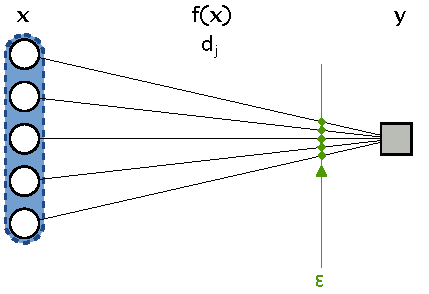
\includegraphics{media/pes_network_a.pdf}%
		\caption{Learning decoders}%
	\end{subfigure}%
	\begin{subfigure}{0.5\textwidth}%
		\centering%
		\includegraphics{media/pes_network_b.pdf}%
		\caption{Delta learning rule}%
	\end{subfigure}%
	\caption{Learning decoders $d_i$ \textbf{(a)} and synaptic weights \textbf{(b)} in an NEF network. We would like to learn an unknown function $\vec y = f(\vec x)$ encoded in either the decoding weights $d_i$ or in the weights between two neural populations. Weights are updated according to an error signal $\epsilon(t) = \vec y^\mathrm{d}(t) - y(t)$.}
\end{figure}

We now have a simple learning rule that allows us to learn decoders online -- essentially, we just multiply the neural activity $a_i(x(t))$ with the error $\epsilon(t)$ and then update individual decoder values according to the gradient descent update equation
\begin{align*}
	d_i \gets d_i -\eta \Delta d_i = d_i -\eta \epsilon(t) a_i(t) \,.
\end{align*}
Essentially, if a neuron is active while there is some positive error $\epsilon(t)$, we decrease its influence on the decoding. If there is a negative error $\epsilon(t)$, we increase its influence.

The problem with this equation is that it is not biologically plausible. There are no decoders in the brain, so we need to find a way to update synaptic weights $w_{ij}$ instead of decoders $d_i$.

However, this problem can be easily fixed. Remember that the synaptic weights are given as
\begin{align*}
	w_{ij} &= \big((\vec \alpha \circ \mat E) \mat D\big)_{ij} = \alpha_i \langle \vec e_i, \vec d_j \rangle \,.
\end{align*}
Substituting the decoder update $\Delta d_j$ into this equation (for the scalar case) gives us
\begin{align*}
	\Delta w_{ij} &= \alpha_i e_i \Delta d_j = - \eta \big( \alpha_i \epsilon(t) e_i \big) a_j(t) \,.
\end{align*}
For vectorial quantities $\vec x$ (i.e., $d > 1$) this just turns out to be
\begin{ImportantEqn}{Prescribed Error Sensitivity (PES) Learning Rule}
\Delta w_{ij} &= \alpha_j e_j \Delta d_i = -\eta \big( \alpha_j \langle \vec \epsilon(t), \vec e_j \rangle \big) a_i(t) \,.
\end{ImportantEqn}
Notice that the term $\big( \alpha_j \langle \vec \epsilon(t), \vec e_j \rangle \big)$ looks very much like the linear part of the current-translation function in the NEF encoding equation. In particular, we are treating the error $\epsilon(t)$ as if it was an input $\vec x(t)$ -- and in a sense it is exactly that -- a so called \enquote{modulatory} input.

As it turns out, such modulatory inputs exist in the brain in the form of dopaminergic synapses, which enable synaptic plasticity in the post-synapse.

\begin{figure}[p]
	\centering
	\begin{subfigure}{\textwidth}
		\centering
		\includegraphics{media/learning_network.pdf}
		\caption{Network used in the experiments depicted below}
	\end{subfigure}
	\begin{subfigure}{\textwidth}
		\centering
		\includegraphics{media/pes_communication_channel_example.pdf}
		\caption{Learning $f(x) = x$}
		\label{fig:pes_communication_channel_example}
	\end{subfigure}
	\begin{subfigure}{\textwidth}
		\centering
		\includegraphics{media/pes_square_example.pdf}
		\caption{Learning $f(x) = x^2$}
		\label{fig:pes_square_example}
	\end{subfigure}
	\caption{\textbf{(a)} Network used for the learning experiment below. Blue boxes correspond to spiking neuron populations of $100$ neurons each. The learning rate is $\eta = 5 \times 10^{-5}$. \textbf{(b, c)} Learning different functions $f$ using the PES learning rule. Blue lines correspond to the decoding from the first neuron population representing $x$, orange lines correspond to the decoding from the second neuron population representing $y = \hat f(x)$. The black line corresponds to the optimal target $f(x)$. \CodeLink{lecture_08/media/code/pes_learning_rule_example.ipynb}}
	\label{fig:pes_learning_network}
\end{figure}

\subsection{Example: Supervised Learning of Functions $f$}

\Cref{fig:pes_learning_network} shows an example of learning a function $f(x) : \mathbb{R} \longrightarrow \mathbb{R}$, with an \enquote{artificially} created error signal $\epsilon(t)$, where \enquote{artificially} refers to the signal being generated outside of the system. As clearly visible in \cref{fig:pes_communication_channel_example}, we are able to quickly learn a communication channel, i.e., $f(x) = x$, between two neuron populations.

Learning a more complex function such as $f(x) = x^2$ works as well, as depicted in \cref{fig:pes_square_example}. However, notice that learning progresses much slower in the second case. Correspondingly, we should note that not only the learning rate $\eta$ plays a role in how fast a function is being learned, but also the \enquote{complexity} of the function that is being learned.

\Note{We will have a closer look at why some functions may be harder to learn than others in the next lecture, when we analyse representations.}

\Note{Given an appropriate learning rate $\eta$ and a long enough training period, learning a function in this way will often result in a smaller error than computing the decoders offline, the reason being that the PES rule has access to the actual spike data instead of \enquote{just} the rate approximation.}

\subsection{Example: Classical Conditioning}

\begin{figure}[p]
	\centering%
	\begin{subfigure}{0.5\textwidth}%
		\centering%
		\includegraphics[scale=0.85]{media/classical_conditioning_a.pdf}%
		\caption{Before conditioning}%
		\label{fig:classical_conditioning_a}
	\end{subfigure}%
	\begin{subfigure}{0.5\textwidth}%
		\centering%
		\includegraphics[scale=0.85]{media/classical_conditioning_b.pdf}%
		\caption{After conditioning}%
		\label{fig:classical_conditioning_b}
	\end{subfigure}\\[0.5cm]
	\begin{subfigure}{\textwidth}%
		\centering%
		\includegraphics[scale=0.85]{media/conditioning_network.pdf}%
		\caption{Network model}
		\label{fig:conditioning_network}
	\end{subfigure}\\[0.5cm]
	\begin{subfigure}{\textwidth}
		\centering
		\includegraphics{media/classical_conditioning_experiment.pdf}
		\caption{Neural network implementing classical conditioning}
		\label{fig:classical_conditioning_experiment}
	\end{subfigure}
	\caption{Classical conditioning experiment. \textbf{(a, b)} Illustration of classical conditioning. An unconditioned stimulus (US, smell of cheese) causes an unconditioned response (UR, mouse is salviating). Paring a neutral conditioned stimulus (CS, light) with the unconditioned stimulus causes the animal to produce a conditioned response (CR). Adapted from \href{https://commons.wikimedia.org/wiki/File:Classical_conditioning_-_extinction.svg}{Wikimedia}. \textbf{(c)} Network model using the PES learning rule to implement classical conditioning.  \textbf{(d)} Graphs showing the values represented by the individual populations.}
	\label{fig:classical_conditioning}
\end{figure}

As mentioned, the above example relies on an \enquote{outside} error signal $\epsilon(t)$. That is, the error signal is produced by the \enquote{environment} that had knowledge about the function $f$ that we wanted to learn. That is, of course, unrealistic. What we would like to have is a system that internally generates the error signal $\epsilon(t)$. One example where we can clearly see how such an error signal could be computed within a neural system itself is classical conditioning.

Classical conditioning is a phenomenon observed in human- and non-human animals, colloquially known through research performed by Ivan Pavlov on dogs (\enquote{Pavlov's dog}).

The general experimental setup is the following. An animal \enquote{unconditonally} (i.e.,~without initial training) responds to a stimulus. In Pavlov's original experiment the unconditional stimulus is the smell of meat presented to a dog (US), that then starts to produce saliva (UR). Another well-studied example is the eye-blink reflex: here, an animal blinks whenever a \enquote{puff} of air is directed at their cornea. This stimulus-response pair is called \enquote{unconditioned stimulus} (US) and \enquote{unconditioned response} (UR). See also \cref{fig:classical_conditioning_a}.

If the unconditioned stimulus is paired with a so called conditioned stimulus (CS) (for example a tone, or a flash of light), the animal gradually learns to associate the conditioned stimulus with the unconditioned stimulus and will produce a conditioned response (CR) mimicking the unconditioned response even in the absence of the unconditioned stimulus (\cref{fig:classical_conditioning_b}).

One possible implementation of classical conditioning using the PES learning rule is depicted in \cref{fig:conditioning_network}. As visible, the system solely receives two modalities as sensory input. We also see the phenomenon of extinction in that example implementation. Note that this might also be understood as a kind of self-supervised learning because the system internally generates the error signal.

\section{Unsupervised Learning}

Internal generation of error signals, as in the classical conditioning example, is often considered a type of unsupervised learning -- although it sits somewhat on the boarder of the supervised and unsupervised dichotomy. Another way to eliminate the need for an external error signal is to not define an explicit target signal $\mat y^\mathrm{d}(t)$ at all, but to instead try to learn structure inherent to samples of data $\vec x_k$ without any external guidance. Often, what we would like to accomplish is some sort of \emph{dimensionality reduction}. That is, we would like to map each high dimensional datum $\vec x_k$ onto a low dimensional space $\vec \lambda$ (the so called \enquote{latent space}), where each dimension in the low dimensional space has some dimension that intrinsically describes the data.

As with supervised learning, the assumption is that there exists a ground-truth function
\begin{align*}
	f^{-1}_\mathrm{GT}(\vec \lambda) : \mathbb{R}^{d'} \longrightarrow \mathbb{R}^d \text{, with } d' \ll d \text{ and } f^{-1}_\mathrm{GT}(\vec \lambda_k) = \vec x_k + \text{ noise} \,.
\end{align*}
That is, we assume that the high-dimensional samples $\vec x_k$ we observe are actually the result of a process that only depends on a few variables $\vec \lambda$. Essentially, we introduce an implicit error signal which is the difference between the high-dimensional and (reconstructed) low-dimensional representations.

\Example{\emph{Faces.} For a moment, think about a set of greyscale photographs of faces. Naturally, we could describe each of these photographs as a vector of pixel intensities $\vec x_k \in \mathbb{R}^d$, where $d$ is the product of the width and height of the photographs in number of pixels. Typically, $d$ would be on the order of magnitude of a few thousand (i.e., for a $32 \times 32$ pixel image we have $d = 1024$) to a few million ($d = 20\times10^6$ for a \enquote{20 megapixel} image).
	
However, we could try to convince ourselves that the most prominent properties of a face can be reduced onto a few dozen dimensions (a good analogy being the character editors present in popular role-playing computer games):
\begin{multicols}{2}
\begin{itemize}
	\item Ratio between width and height
	\item Relative eye, mouth, nose distance
	\item Nose, eye, mouth shape
	\item Emotion (happy, angry, surprise, \textellipsis)
	\item Skin tone
	\item Hair color and length
\end{itemize}
{\centering
\includegraphics[height=4cm]{media/face_database_2.pdf}\\}
{\small\stepcounter{figure}\textbf{Figure \arabic{figure}.} Excerpt from the face database used in the following experiments. \href{http://pics.stir.ac.uk/2D_face_sets.htm}{Source}}
\end{multicols}
We could devise a way to quantify each of these features in terms of a scalar value $\lambda_i$. Then, we can write a function $f$ that takes a parameter vector $\vec \lambda$ and outputs a face.

The goal of unsupervised learning is to automatically determining both the parameter space $\vec \lambda$, as well as an encoder $f$ (encoding a set of parameters $\vec \lambda$ into the high dimensional space), and the decoder $f^{-1}$ (estimating $\vec \lambda$ given a high-dimensional input).
}

\subsection{Autoencoders}

An extremely powerful dimensionality reduction method are so called autoencoders. The idea is to build a neural network $f(\vec x, \vec w)$ such that after training $f(\vec x; \vec w) = \vec x$, i.e., the output of the network is equal to its input. Crucially however, the network posesses a so called \enquote{information bottleneck}, a neural layer with just a few dimensions $d' \ll d$. The activities of the neurons in this layer correspond to the latent space $\vec \lambda$. See \cref{fig:autoencoder} for a sketch of an autoencoder network.

To train an autoencoders we optimize the loss $\| f(\vec x; \vec w) - \vec x \|$. Since the desired output is just the input, this can be interpreted as a supervised learning problem. Correspondingly, we can do stochastic gradient descent using back-propagation (see above). This method can yield quite impressive results (see this \YouTube{Q1XuXwPVFko} for varying $\lambda$ in a trained autoencoder).

Unfortunately, back-propagation in a multi-layer network is biologically implausible (cf.~\cite{hunsberger2018spiking}). Correspondingly this method does not really qualify for our purpose of building a brain model.

\Aside{\emph{Regularisation of $\vec \lambda$ -- Variational Autoencoders.}
One caveat when training autoencoders is overfitting (i.e., a small error on the training dataset $X$, but bad generalisation). While this problem is of course not exclusive to autoencoders, they tend to exhibit this behaviour in a particularly interesting way. Even with a bottleneck dimension of $d' = 1$, the training error goes to zero -- the dataset is somehow being compressed into a single scalar~$\lambda_1$. Of course, this does not mean that the autoencoder actually learned something useful, but merely that the encoding function $f(\lambda; \vec w)$ \enquote{remembers} the entire dataset in its connection weights $\vec w$ and that $\lambda_1$ is effectively an index into our datapoints.

Crucially, as impressively shown by Piantadosi, 2018 \cite{piantadosi2018one} (see below) this may happen when learning a function with just a single parameter $w$, since a single real number can encode an infinite amount of information (or up to 64 bit of information when using a double precision floating point number on a computer).

To prevent this from happening, we need to apply some regularisation to the bottleneck of the autoencoder, either by discretising $\lambda$ to much less than 64 bit, adding noise, or treating $\lambda$ as parameters of a probability distribution from which we sample the input to the encoding layer. The latter method is known as a \emph{Variational Autoencoder}.

{\centering\includegraphics{media/piantadosi_2018_one_parameter_is_always_enough.pdf}\\}
{\small\stepcounter{figure}\textbf{Figure \arabic{figure}.} Compressing a large training set $\mat X$ into a single parameter $\theta$. The depicted $f(x, \theta)$ \enquote{stores} two different datasets $X$ in a single parameter $\theta \in [0, 1]$ each. Figure copied from \cite{piantadosi2018one}.}
}

\begin{figure}
	\centering
	\includegraphics[scale=0.833]{media/autoencoder.pdf}
	\caption{Network diagram of a potential autoencoder architecture. A neural network is trained to reproduce a $d$ dimensional input $\vec x_k$ while feeding the data through a $d'$ dimensional bottleneck with $d' \ll d$. Note that $d$ would usually be much larger than what is shown here.}
	\label{fig:autoencoder}
\end{figure}

\subsection{Principal Component Analysis}

An interesting concept that -- as we will see -- is directly related to unsupervised learning in biologically plausible neural networks, is the so called Principal Component Analysis, often referred to as PCA. In short, the PCA computes a linear basis transformation $\mat T$ that transforms the input samples $\vec x_k$ in such a way that the most information (in terms of variance) is explained by the first dimensions of the resulting $\lambda_k$.

\paragraph{Basis Transformation}
In order to understand this a little better, let's first define what a \emph{basis transformation} is. Let $\mat T \in \mathbb{R}^{d \times d}$ be an orthogonal (aka orthonormal) matrix, that is $\mat T \mat T^\T = \mat T^\T \mat T = \mat I$, then $\mat T$ can be seen as a so called \enquote{basis transformation}. The mathematical term for an orthogonal transformation matrix is \emph{rotation}. Rotations are quite intuitive in two and three dimensions (they do exactly what their name suggests, i.e.,~they change the orientation of points in space without changing their distance), where we can easily visualise rotations, but we can no longer to so for $d > 3$. Nevertheless, it holds
\begin{align*}
	\vec \lambda = \mat T \vec x \,, \quad \text{ and }\quad \vec x = \mat T^\T \vec \lambda \,, && \text{ where } \mat T \in \mathbb{R}^{d \times d} \, \text{ and } \vec x, \vec \lambda \in \mathbb{R}^d \,.
\end{align*}
Note the equalities: the transformation from $\vec x$ to $\lambda$ is \emph{lossless}. We can go from one space to the other without losing any information.

\Note{We have already seen some basis transformations in this course. For example, the Discrete Fourier Transformation (DFT), the Discrete Cosine Transformation (DCT), and the Laplace transformation can all be defined in terms of such a matrix $\mat T$.}

\paragraph{Computing Principal Components}
The idea behind the PCA is the following. What if we could find the transformation $\mat T$ that packs the most \enquote{information} into the first dimensions of our rotated vectors $\lambda$? Then, we might be able to do the following.
\begin{enumerate}
	\item \textbf{Compression}\\
	If we only look at the first $d'$ dimensions of $\lambda$, i.e.,~discard (set to zero) all dimensions $i > d'$, we might still be able to get a good (though no longer lossless) reconstruction of~$\vec x$.
	\item \textbf{Interpretation}\\
	If the first $d'$ dimensions contain the \enquote{most information}, these dimensions could have interesting semantics.
\end{enumerate}
One way to define \enquote{the most information}, is by the variance of our dataset along a certain axis. Hence, for the first PCA dimension, we want to project our dataset $X$ onto a vector $\vec t_1$ such that the variance is maximal
\begin{align*}
	\vec t_1 &= \arg\max_{\vec t_1} \mathrm{var}\big(\vec t_1 \mat X\big) \,, \text{ where } \vec t_1 \in \mathbb{R}^{1 \times d} \text{ and } \mat X \in \mathbb{R}^{d \times N} \,.
\end{align*}
We can find \enquote{the second best} transformation vector $\vec t_2$ by subtracting the data that is aligned with $\vec t_1$ from our dataset and then repeating the above process
\begin{align*}
	\vec t_2 &= \arg\max_{\vec t_2} \mathrm{var}\big(\vec t_2 ( \mat X - \vec t_1^\T \vec t_1 \mat X) \big) \,, \text{ where } \vec t_1 \in \mathbb{R}^{1 \times d} \text{ and } \mat X \in \mathbb{R}^{d \times N} \,.
\end{align*}
This process can be repeated $d$ times, giving us vectors $\vec t_1, \ldots, \vec t_d$.

\paragraph{Eigendecomposition}
Solving the above optimization problem as we did multiple times before, one can show, that the above process is equivalent to computing the Eigenvectors $\mat V$ of the covariance matrix $\mat C$ of $\mat X$, sorted by the magnitude of the Eigenvalues $\lambda_i$. That is, the Eigenvector with the largest Eigenvalue is equal to $\vec t_1$, the Eigenvector with the second-largest Eigenvalue is equal to $\vec t_2$, and so on.

The covariance matrix of $\mat X$ is given as
\begin{align*}
	\mat C = \frac{\big(\mat X - \bar{\vec x}\big)^\T \big(\mat X - \bar{\vec x}\big)}{N - 1} \,,
\end{align*}
the Eigenvalues and Eigenvectors are part of the so called Eigendecomposition. For any real symmetric square matrix $\mat C$ with linearly independent eigenvectors
\begin{align*}
	\mat C = \mat V \mat \Lambda \mat V^\T \,,
\end{align*}
where $\mat V$ is an orthogonal matrix, and $\Lambda$ is a diagonal matrix of Eigenvalues.

\cprotect\Python{In Python using \texttt{numpy}, the PCA can be computed as follows
\begin{lstlisting}[language=python]
def PCA(X): # X: N x d matrix
    N, d = X.shape 
    X_cen = X - np.mean(X, axis=0)
    C = (X_cen.T @ X_cen) / (N - 1)
    L, V = np.linalg.eigh(C) # "eigh" is faster than "eig" for symmetric matrices
    return V.T[::-1, :] # d x d matrix
\end{lstlisting}}

\newpage

\cprotect\Note{\emph{Computing the PCA using Singular Value Decomposition (SVD).}
An alternative to computing the PCA using Eigen decomposition is to use the so called \enquote{Singular Value Decomposition} (SVD) instead. The SVD is a generalised form of the Eigen decomposition for non-square matrices. This saves having to compute the covariance matrix $\mat X$, making the above code a wee bit shorter:
\begin{lstlisting}[language=python]
def PCA_SVD(X): # X: N x d matrix
    return np.linalg.svd(X - np.mean(X, axis=0))[2]
\end{lstlisting}
To see why this works, consider that the SVD decomposes a matrix $\mat X$ into a product of three matrices $\mat U$, $\mat S$, $\mat V$ with $\mat X = \mat U \mat S \mat V^\T$, where $\mat S$ is a diagonal matrix of the so called \emph{singular values}, and both $\vec U$ and $\vec V$ are orthogonal matrices.

Assume that we have the SVD of the centered data matrix $\mat X$ with
\begin{align*}
	(\mat X - \bar{\vec x}) &= \mat U \mat S \mat V^\T \,.
\end{align*}
Comparing this to the Eigen decomposition of the covariance matrix $\mat C$ we get
\begin{align*}
	\mat C &= \frac{(\mat X - \bar{\vec x})^\T (\mat X - \bar{\vec x})}{N - 1}
	        = \frac{\mat V \mat S \mat U^\T \mat U \mat S \mat V^\T}{N - 1}
	        = \mat V \frac{\mat S^2}{N - 1} \mat V^\T¸
	        = \mat V \mat L \mat V^\T \,.
\end{align*}
Hence the matrix $\mat V$ of the SVD of the centered data matrix $\mat X - \bar{\vec x}$ is equivalent to the matrix $\mat V$ of the Eigen decomposition of the covariance matrix of $\mat X$.}

\subsection{Example: Applying the PCA to Faces}

\begin{figure}[p]
	\begin{subfigure}{0.5\textwidth}
		\centering
		\includegraphics[width=0.8\textwidth]{media/eigenfaces_normal_basis.pdf}
		\caption{Normal basis $\mat I$}
		\label{fig:eigenfaces_normal_basis}
	\end{subfigure}
	\begin{subfigure}{0.5\textwidth}
		\centering
		\includegraphics[width=0.8\textwidth]{media/eigenfaces.pdf}
		\caption{PCA basis $\mat T$}
		\label{fig:eigenfaces}
	\end{subfigure}
	\begin{subfigure}{\textwidth}
		\centering
		\includegraphics[scale=0.9]{media/eigenfaces_dim_2_3.pdf}		
		\caption{Images plotted along the magnitude of the third and fourth principal components.}
		\label{fig:eigenfaces_dim_2_3}
	\end{subfigure}
	\caption{Principal component analysis of a set of faces. \textbf{(a)} Orthonormal basis used to represent pixel data. Each vector component in $\vec x_k$ corresponds to exactly one pixel. \textbf{(b)} Orthonormal basis vectors computed by the PCA. Each vector component in $\vec \lambda$ affects all pixels. Any image in the dataset $\mat X$ can be reconstructed by forming a weighted sum of these \enquote{basis images}. \textbf{(c)} Plotting a set of images according to the magnitude of their third and fourth principal component. Images appear to be approximately spatially arranged by emotion. \CodeLink{lecture_08/media/code/eigenfaces.ipynb}}
	\label{fig:pca_faces}
\end{figure}

An example applying the PCA to a set of faces is shown in \cref{fig:pca_faces}. The face database (available \href{http://pics.stir.ac.uk/2D_face_sets.htm}{here}), contains 84 grayscale images of 12 women with 7 different facial expressions. The images are normalised such that the eyes are located at approximately the same pixel location. Each image is $45 \times 60$ pixels large (resolution quartered compared to the original dataset), corresponding to a total dimensionality of $d = 2700$.

Since the individual principal components $\vec t_1, \ldots, \vec t_d$ are $2700$ dimensional vectors, we can draw them as images in the same way we can draw the original $\vec x_k$ as images (\cref{fig:eigenfaces}). In this particular example, these images are known as \enquote{Eigenfaces}. The first principal component vectors correspond to \enquote{average} faces in the dataset. That is, each component of $\vec \lambda_k$ affects the entire image -- compare this to vector components in the original image $\vec x_k$ which only affect a single pixel (cf.~\cref{fig:eigenfaces_normal_basis}). In particular, the first two basis vectors and the corresponding latent space dimensions $\lambda_1$ and $\lambda_2$ encode information about the skin tone and the background/hair color. Subsequent principal components weight information from individual face areas and can be interpreted as encoding the facial expressions of the subjects (\cref{fig:eigenfaces_dim_2_3}).

Hence, the PCA seems to act as an unsupervised learner. We are able to automatically extract high-level semantic features from a set of data points without specifying what we were looking for -- the individual principal components correspond to common patterns in the dataset $\vec X$.

\newpage

\Note{\emph{Machine learning and human data.} Be careful when using (unsupervised) machine learning on any data related to humans! In this example, the PCA algorithm determined on its own that skin color (principal component coefficient $\lambda_1$) contains the \enquote{most information} about the photos. This makes sense from a purely visual perspective (after all, most pixels in the photo depict skin). Luckily, the result of the PCA can be easily analysed as shown in \cref{fig:pca_faces}. Hence, we can decide not to use this dimension for subsequent processing. However, performing such analyses is much more difficult in more complex machine learning algorithms (i.e.,~\enquote{deep neural networks}). The machine might implicitly discriminate against certain groups of people without the engineers building the system noticing.}

\Note{\emph{Limitations of the PCA.} While the PCA seems to be quite powerful in the above example, it is generally inferior to an autoencoder. We are restricting ourselves to linear transformations $\mat T$. In many cases, nonlinear transformations are required to extract useful information from datasets.}

\subsection{Hebbian Learning}

We have now discussed Principal Component Analysis, but it is still unclear how this relates to biology.
One of the first attempts at characterising learning in biological systems was made by Donald Hebb in his 1949 book \enquote{The organization of behavior} \cite{hebb1949organization}:
\begin{quotation}
	When an axon of cell $A$ is near enough to excite a cell $B$ and repeatedly or persistently takes part in firing it, some growth process or metabolic change takes place in one or both cells such that $A$'s efficiency, as one of the cells firing $B$, is increased.
\end{quotation}
An often made qualitative summary of the above statement is \enquote{what fires together wires together}, that is, the synaptic strength $w_{ij}$ between a post-neuron $i$ and a pre-neuron $j$ increases. We can easily turn this into a mathematical equation:
\begin{ImportantEqn}{Hebbian Learning}
	\Delta w_{ij} &= \eta a_i a_j
	\label{eqn:hebbian_learning}
\end{ImportantEqn}
Evidence for this rule has (among others) been gathered by Eric Kandel in the synaptic connections responsible for the \enquote{siphon withdrawal reflex} in the sea slug \emph{Aplysia Californica}.

There are two problems with this equation. First, it is \emph{unstable} -- the weights $w_{ij}$ tend to grow to infinity. Correspondingly, this rule is never used directly, and instead, there are several learning rules based on \cref{eqn:hebbian_learning} that solve this problem. We will discuss some of these learning rules below. Depending on how the stabilisation of the equation is performed, these learning rules compute the principal components online.

Second, the equation does not take \emph{causation} into account (i.e., which neuron caused the firing of the post neuron). This is solved by a \enquote{Spike-Time Dependent Plastiticy}, which we will also discuss below.

\subsection{Stable Hebbian Learning}

\begin{figure}
	\centering
	\includegraphics{media/hebbian_learning_example.pdf}
	\caption{Normalised Hebbian Learning, or, equivalently, the Oja rule. Visualisation of the weight vector $\vec w_i$ connecting from a pre-population of $2700$ neurons representing individual pixel intensities onto a single post-neuron. The initially random weight vector approaches the first principal component over time (left to right, $t$ corresponds to iterations; compare to \cref{fig:pca_faces}). \CodeLink{lecture_08/media/code/bcm_example.ipynb}}
	\label{fig:hebbian_learning_example}
\end{figure}

\paragraph{Normalised Hebbian Learning}
One way to prevent the synaptic weights from diverging is to force normalisation of the post-synaptic weights in the post-neuron $i$, that is
\begin{align*}
	\Delta w_{ij} &= \eta a_i a_j \,, & \text{ where } \vec w_{i} \gets \frac{\vec w_i + \Delta \vec w_{i}}{\|\vec w_i + \Delta \vec w_{i}\|} \text{ in every time step}\,.
\end{align*}
This way, the overall magnitude of the synaptic weight vector $\vec w_{i}$ describing all connections to the post-neuron $i$ is limited. This could be interpreted as a \enquote{homeostasis} mechanism in the post-neuron. As mentioned above, one can show that --- under the assumption of a linear post-neuron model -- the weights $\vec w_i$ converge to the first principal component of the pre-population activity (see also \cref{fig:hebbian_learning_example}). Several methods exist that ensure learning of more principal components, however, this is an active field of research.

From a biological perspective, the above equation is a little implausible in that it assumes that the post neuron is able to compute a vector norm. Correspondingly, several alternative rules exist that implicitly incorporate the normalisation into the weight-update.

\paragraph{Oja rule}
The Oja rule (proposed by Erkki Oja, 1982) can be derived from the above \enquote{normalised} equation and is equivalent to it for a post-neuron with a linear activation function
\begin{align*}
\Delta w_{ij} &= \eta \big(a_i a_j - a_i^2 w_{ij}\big) \,.
\end{align*}
Instead of requiring repeated computation of the vector norm $\|\vec w_i\|$, this rule ensures stability by subtracting the weighted squared post-neuron activity. This rule can be used as a learning rule in Nengo connection objects.

\paragraph{BCM Rule}
The BCM (Bienenstock, Cooper \& Munro, 1981) rule balances the weight update by adding a target firing rate $\theta$ -- if the post neuron is below that firing rate, the weight is increased, otherwise the weight is being decreased:
\begin{align*}
	\Delta w_{ij} &= \eta a_j a_i (\theta - a_i) \,.
\end{align*}
Often, $\theta$ is modelled as an averaged function of the past neural activity -- this way, the post-neuron attempts to maintain a more or less steady firing rate. This rule can also be used as a learning rule in Nengo connection objects.

\newpage

\Note{\emph{Unsupervised learning from the perspective of individual neurons.} Another, perhaps overly metaphorical way to look at unsupervised learning is from the perspective of an individual neuron. Individual neurons have very little information about global information processing in the brain---all they \enquote{know} about the world are the firing patterns of their respective pre-neurons.
	
Still, the \enquote{goal} of an individual neuron could be seen as being \enquote{useful} to the organism as a whole. While a precise definition of \enquote{useful} is hard, certainly, a neuron not firing at all or just firing all the time is not very useful. Also, a neuron just repeating what their neighbouring neurons are doing might not be very helpful to the system as a whole---this is why we often find so called \enquote{lateral inhibition} between neighbouring neurons, acting as a sparsification of the population response.

One possible definition of \enquote{usefulness} is to extract as much information as possible from pre-synaptic events, accounting for what neighbouring neurons population are already sensitive to. In other words, a neuron should seek to extract patterns in the pre-neuron activities that other neurons in the population are not sensitive to, for example by each neuron being sensitive to a different principal component of the pre-population.

There are many different ways of characterising the amount of information in a post-neuron, relative to the pre-neuron activities. In case you are interested in this, have a look at Chapter 4 of Dayan and Abbott, \emph{Theoretical Neuroscience}, 2001 \cite{abbott2001theoretical}.}

\subsection{Spike-Time Dependent Plasticity (STDP)}

Note that Hebb's original theory quoted above is a little more precise than what is expressed in \cref{eqn:hebbian_learning}. The term \enquote{takes part in firing it} suggests that there must be a \emph{causal} relationship between the pre-neuron activity $a_j^\mathrm{pre}$ and the post-neuron activity $a_i^\mathrm{post}$. Here, \enquote{causal} means that the pre-neuron must contribute to the firing of the post neuron; in other words, two neurons just \enquote{randomly} firing independently of each other will on average not cause an increase in synaptic strength.

One way to incorporate such a causal relationship into the learning rule is to consider individual spike times. If post-neuron $B$ spikes \emph{before} pre-neuron $A$ spikes, then neuron $A$ cannot have \emph{caused} the spike. Conversely, if neuron $B$ spikes shortly after neuron $A$, then there it is more likely that $A$ caused the spike in $B$.

This is commonly modelled as \enquote{Spike-Time Dependent Plasticity} (STDP) \cite{sjostrom2010spiketiming}. Let $t^\mathrm{pre,j}_1, \ldots, t^\mathrm{pre,j}_N$ denote the spike times of the pre-neuron $A$, and $t^\mathrm{post,i}_1, \ldots, t^\mathrm{post,i}_{N'}$ denote the spike times of the post-neuron $B$. Then, the weight update is given as
\begin{align*}
	\Delta w_{ij} = \eta \sum_{k = 1}^N \sum_{\ell = 1}^{N'} W\left(t^\mathrm{post,i}_k - t^\mathrm{pre,j}_\ell\right) \,.
\end{align*}
A popular choice for $W(\theta)$ (see \cref{fig:stdp}) is
\begin{align*}
	W(\theta) = \begin{cases}
		\alpha^+ e^{-\theta / \tau^+}¸& \text{if } \theta > 0 \,,\\
		-\alpha^- e^{-\theta / \tau^-}& \text{if } \theta \leq 0 \,,
	\end{cases}
\end{align*}
where the time constants $\tau^+$ and $\tau^-$ are typically in the range of \SI{10}{\milli\second}. There is strong experimental support for this type of learning -- see \cite{sjostrom2010spiketiming} for more details. It has been suggested that, in fact, the STDP and BCM rules capture the same phenomena under appropriate interpretations of `activity' as post-synaptic filtered spikes \cite{bekolay2011masters}.

\begin{figure}
	\centering
	\includegraphics{media/stdp.pdf}
	\caption{The STDP function $W(\theta)$. If the pre-spike occurs after the post-spike ($\theta < 0$), the synaptic weight decreases. Otherwise, if the pre-spike occurs before the post-spike ($\theta > 0$) the synaptic weight increases.}
	\label{fig:stdp}
\end{figure}


\printbibliography

\end{document}

